\section{Task 2}
Die Abbildungen \ref{fig::avgtime Depth2.1} und \ref{fig::avgtime Depth 2.2} zeigen die durchschnittlichen Bedenkzeiten pro Zug auf zehn verschiedenen Maps. Die Daten wurden erhoben indem jeweils ein gesamtes Spiel auf der Map gespielt wurde mit eingeschalteten Performance-Logging und anschließend der ausgegebene Log geparsed wurde.\\
\begin{figure}[h]
	\begin{center}
		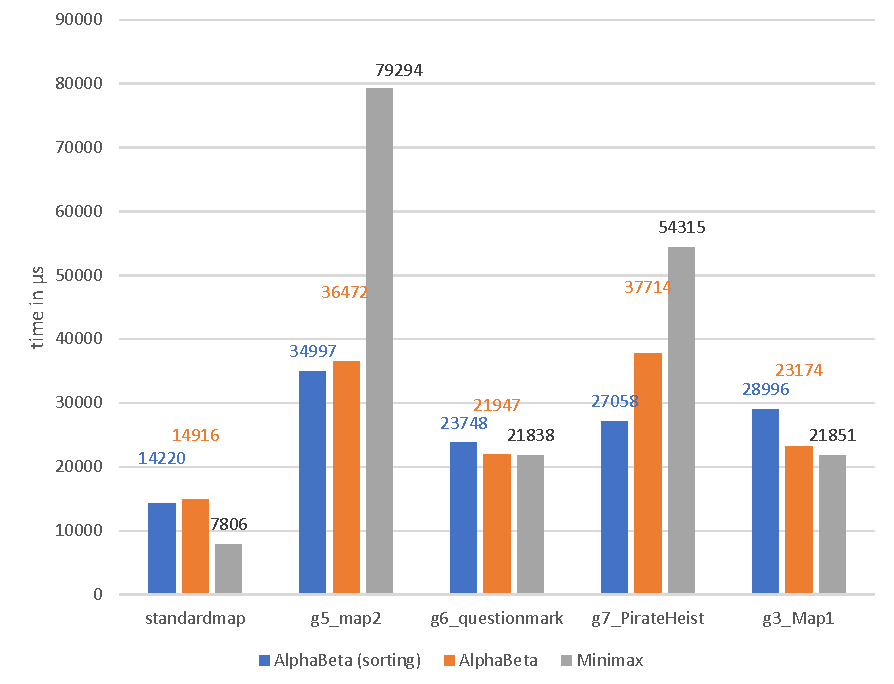
\includegraphics[scale=0.5]{Depth_2_1_avgtime.pdf}
		\caption{Durchschnittszeit bei Tiefe 2 (1/2)}
		\label{fig::avgtime Depth2.1}
	\end{center}
\end{figure}
\begin{figure}[h]
	\begin{center}
		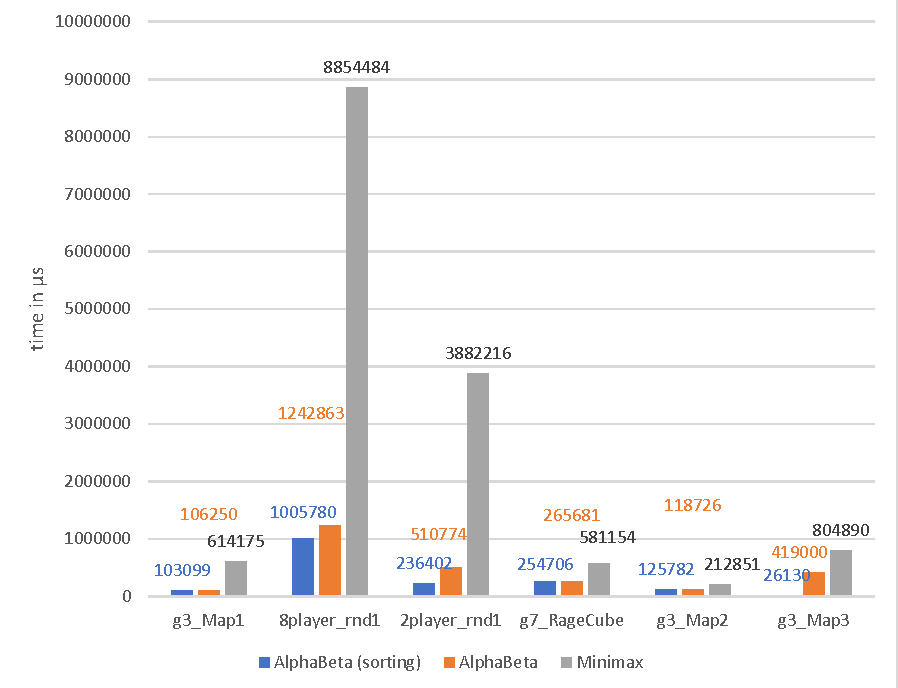
\includegraphics[scale=0.5]{Depth_2_2_avgtime.pdf}
		\caption{Durchschnittszeit bei Tiefe 2 (2/2)}
		\label{fig::avgtime Depth 2.2}
	\end{center}
\end{figure}
Es war zu erwarten, dass die durchschnittliche Bedenkzeit beim Alpha-Beta Algorithmus mit Zugsortierung stets geringer ist, als die ohne Sortierung. Leider entsprechen unsere Messungen nicht ganz den Erwartungen. Die Bedenkzeiten liegen sehr oft auf gleicher Höhe. Eine enorme Verbesserung erzielen wir nur auf der 2-Spieler Random-Map sowie auf der Map3 unserer Gruppe. Besonders erschreckend ist das Messergebnis auf der Standardmap sowie auf g6-questionmark. Dort scheint der Minimax \textbf{schneller} zu sein als der Alpha-Beta und die Zugsortierung ist eine Einbuße von Performance. Auf der Suche nach einer Erklärung sind wir auf folgende Punkte gestoßen:
\begin{enumerate}
\item[1.] \textbf{Die verschiedenen Suchverfahren hatten keine identischen Spiele:} Das passiert durch eine unterschiedliche Zugsortierung und bei gleichwertigen Zügen bzgl. der Bewertungsfunktion. Ein unterschiedlicher Spielverlauf kann unterschiedliche Komplexität mit sich führen und somit eine unterschiedliche Durchschnittszeit. Jedoch ist es sehr unwahrscheinlich, dass dieser Einfluss die Bedenkzeit des Alpha-Beta Algorithmus über die des MiniMax bringt.
\item[2.] \textbf{Fehler in der Datenerhebung:} Wir können nicht komplett ausschließen, dass die Messung der Performance unentdeckte Fehler beherbergt.
\item[3.] \textbf{Fehler in der Implementierung:} Der Vollständigkeit halber sei dieser Punkt ebenfalls aufgeführt, wobei einige nachträgliche Tests darauf hindeuten, dass die Implementierung in Ordnung ist.
\end{enumerate}
Da unsere Zugsortierung Züge mit speziellen Effekten ordnet (z.B. Override-uses oder Bonus-Felder), verliert sie jegliche Wirkung auf Karten, auf denen besonders wenige Spezial-Felder oder Override-stones zur Verfügung stehen. Dennoch sollte sie insgesamt eine größere Auswirkung haben.

%\begin{figure}[h]
%	\begin{center}
%		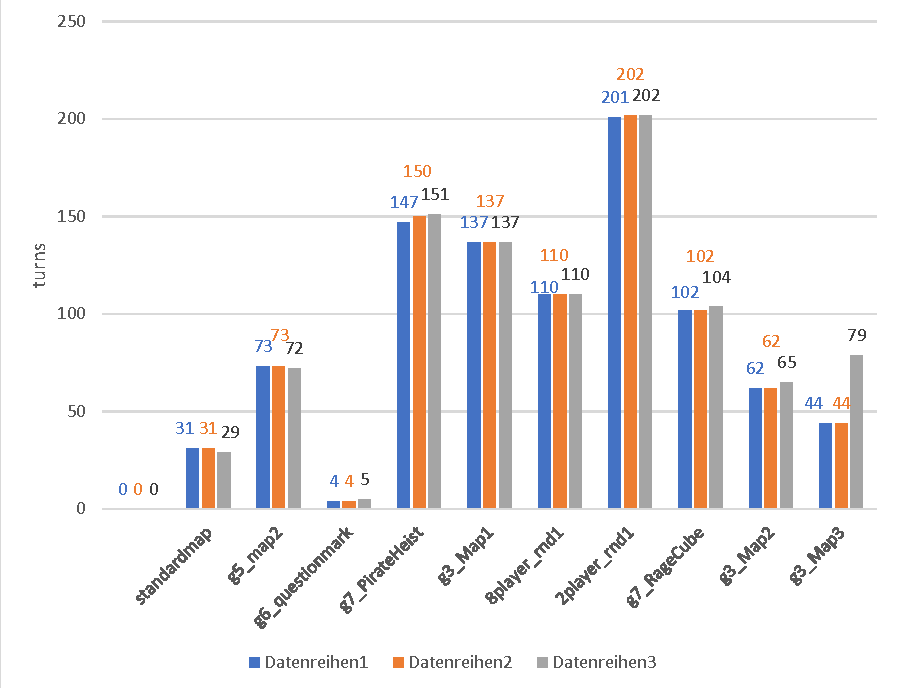
\includegraphics{Depth_1_turns.pdf}
%		\caption{Anzahl der Züge bei Tiefe 1}
%		\label{fig::turns Depth1}
%	\end{center}
%\end{figure}